% =============================================================================
%  Diagrama de flujo IDC mono-objetivo (IDC-SO), en español, vectorial.
%  Reemplaza a fig_idc_so.jpg (inglés, con erratas). Compilar: pdflatex.
%  Sin babel: con [spanish] los caracteres > y % se vuelven activos y rompen
%  la sintaxis >= de TikZ y los % matemáticos.
% =============================================================================
\documentclass[border=6pt]{standalone}
\usepackage[T1]{fontenc}
\usepackage[utf8]{inputenc}
\usepackage{tikz}
\usetikzlibrary{positioning,shapes.geometric,arrows.meta,calc,backgrounds,fit}

\definecolor{idcblue}{RGB}{31,103,131}
\definecolor{idcpink}{RGB}{244,193,167}

\begin{document}
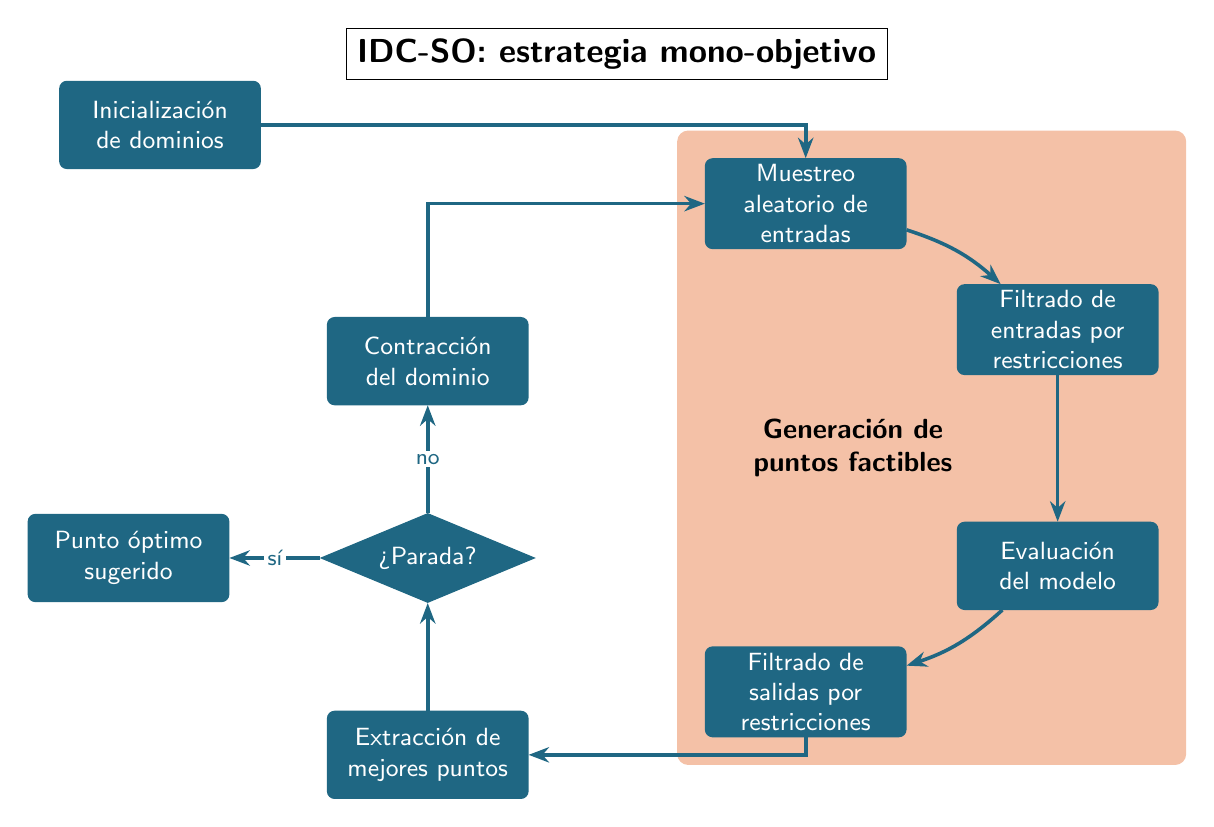
\begin{tikzpicture}[
  font=\sffamily\small,
  >={Stealth[length=3mm]},
  box/.style   = {rectangle, rounded corners=2.5pt, draw=idcblue, fill=idcblue,
                  text=white, align=center, minimum height=11mm, text width=24mm,
                  inner sep=2pt, line width=0.6pt},
  dec/.style   = {diamond, draw=idcblue, fill=idcblue, text=white, aspect=2.4,
                  align=center, inner sep=1pt, text width=18mm, minimum height=11mm},
  fl/.style    = {-{Stealth[length=2.6mm]}, idcblue, line width=1.3pt},
  lab/.style   = {font=\sffamily\footnotesize, fill=white, inner sep=1.2pt},
  title/.style = {draw=black, fill=white, rounded corners=0pt, font=\sffamily\bfseries\large,
                  inner sep=4pt}
]

% --- Título ------------------------------------------------------------------
\node[title] at (8.4,9.3) {IDC-SO: estrategia mono-objetivo};

% --- Contenedor de generación de puntos factibles ---------------------------
\node[box] (mues)  at (10.8,7.4) {Muestreo\\ aleatorio de\\ entradas};
\node[box] (filin) at (14.0,5.8) {Filtrado de\\ entradas por\\ restricciones};
\node[box] (eval)  at (14.0,2.8) {Evaluación\\ del modelo};
\node[box] (filou) at (10.8,1.2) {Filtrado de\\ salidas por\\ restricciones};

\begin{scope}[on background layer]
  \node[fill=idcpink, rounded corners=4pt,
        fit=(mues)(filin)(eval)(filou), inner sep=10pt] (cont) {};
\end{scope}
\node[font=\sffamily\bfseries, align=center, text=black] at (11.4,4.3)
     {Generación de\\ puntos factibles};

% --- Columna izquierda -------------------------------------------------------
\node[box] (init)  at (2.6,8.4) {Inicialización\\ de dominios};
\node[box] (contr) at (6.0,5.4) {Contracción\\ del dominio};
\node[dec] (stop)  at (6.0,2.9) {¿Parada?};
\node[box] (best)  at (6.0,0.4) {Extracción de\\ mejores puntos};
\node[box] (opt)   at (2.2,2.9) {Punto óptimo\\ sugerido};

% --- Flujos del lazo interno (sentido horario) ------------------------------
\draw[fl] (mues)  to[bend left=12] (filin);
\draw[fl] (filin) -- (eval);
\draw[fl] (eval)  to[bend left=12] (filou);

% --- Flujos de control -------------------------------------------------------
\draw[fl] (init.east) -| (mues.north);
% salida del contenedor: baja 90 grados y entra por la derecha de Extracción
\draw[fl] (filou.south) |- (best.east);
\draw[fl] (best.north) -- (stop.south);
\draw[fl] (stop.north) -- node[lab]{no} (contr.south);
\draw[fl] (contr.north) |- (mues.west);
\draw[fl] (stop.west) -- node[lab]{sí} (opt.east);

\end{tikzpicture}
\end{document}
